\cotefile{70}
\scanpage{50}
% L01
2 -- Polyèdres réguliers.

% L02
(Vieille rédaction)

% left edge, faint partly clipped pencil mark
\margin{\unsure{3}}
% archive sheet number: 49

\scanpage{51}
\mspage{\unsure{(47)|(48)}}
% L01-03
2\unsure{-|=}Polyèdres infinis en \unsure{coordonnées|coordonnés|coordonnees} universelles

% L04
(vieille rédaction)
% archive sheet number: 50

\scanpage{52}
% L01-02
$\underline{X}=(\underline{S},\underline{A},\underline{F},\underline{R},\underline{R'},\underline{R''})$ polyèdre combinatoire $\underline{\unsure{\mathscr{R}|\mathcal{R}|R}}$ ens de ses repères.

% L03
$E$ espace affine (proj.) sur $k$ (corps)

% L04
Réalisation géom de $X$
% L05-07
\[
\left\{\begin{aligned}
\varphi_S &: \underline{S}\mathrel{\unsure{-|\longrightarrow}}E\\
\varphi_A &: \underline{A}\mathrel{\unsure{-|\longrightarrow}}\mathrm{Dr}(E)\\
\varphi_F &: \underline{F}\mathrel{\unsure{-|\longrightarrow}}\mathrm{Pl}(E)
\end{aligned}\right.
\]

% L08-09
1°) \unsure{Compatible|Compatibles} avec $R',R''$, donc $R$. On suppose de plus que

% L10-12
2°) a) Si $a\in A$, $s,s'\in S$ les deux sommets incidents $f,f'$ les deux faces incidentes, on a $\varphi_S(s)\ne\varphi_S(s')$, $\varphi_F(f)\ne\varphi_F(f')$

% L13-14
b) Si $s<f$ avec $s\in S$, $f\in F$, et si $a,a'$ sont les deux arêtes entre $s$ et $f$, on a $\varphi_A(a)\ne\varphi_A(a')$.

% L15-16
$\Rightarrow\varphi_S$ détermine $\varphi_A,\varphi_F$ / \unsure{de m.} $\varphi_F$ détermine $\varphi_A,\varphi_S$ / $\varphi_A$ détermine $\varphi_S$ donc $\varphi_F$

% L17-18, cancelled draft sentence
\deleted{Si $X$ est régulier, une telle \unsure{réalisat.|réalisation} \unsure{géom} \uline{\unsure{régulière}}}

% L19-23
\uline{Prop} Soit $\underline{r}_0=(\underline{s}_0,\underline{a}_0,\underline{f}_0)$ un repère de $X$. \unsure{Soit|Les} $\underline{s}_1$ le deuxième sommet de $\underline{a}_0$, $\underline{s}_2$ le deuxième sommet de la 2\textsuperscript{e} arête \inserted{$\unsure{a_1^+|a_0^+}$} \unsure{entre} $\underline{s}_0$ et $\underline{f}_0$, enfin $\underline{s}_3$ le deuxième sommet de la 2\textsuperscript{ième} arête \unsure{au} entre $\underline{s}_0$ et $\underline{f}_1$, la 2\textsuperscript{ième} facette \unsure{passant} par $\unsure{\underline{a}_0|\underline{f}_0}$.

% L24-25
Considérons les images $s_0,s_1,s_2,s_3$ dans $E$. Alors ces pts sont affinement indépendants
% archive sheet number: 51

\scanpage{53}
% L01-07
\uline{Dém} $s_1\ne s_0$ \inserted{et $s_2\ne s_0$} par a) 1°; $a_1\ne a_0$ par b), donc $s_2\notin a_0$, donc $s_0,s_1,s_2$ aff\textsuperscript{t} indép, $f_0$ est le plan qu'ils engendrent. \unsure{De m} \unsure{(en remplaçant|[remplaçant} \inserted{$r_0=(s_0,a_0,f_0)$} par $r_1=(s_0,a_0,f_1)$] on voit que $f_1$ est le plan engendré par $s_0,s_1,s_{\unsure{2|3}}$. Or $f_1\ne f_0$ \deleted{\unsure{(car|(par|par}} par a) 2°, donc $s_3\notin f_0$, donc $s_0,s_1,s_2,s_3$ aff\textsuperscript{t} indép.

% L08-10
\uline{Cor}
\[
\begin{aligned}
a_0&=\mathrm{dr}(s_0,s_1)\\
f_0&=\mathrm{pl}(s_0,s_1,s_2)
\end{aligned}
\mathrel{\big|\!\!\Longrightarrow}
\begin{gathered}
\varphi_A,\varphi_F\ \text{connus quand}\\
\text{on \unsure{connaît|connait} }\varphi_S
\end{gathered}
\]

% L11-15
\unsure{de même}
\[
\begin{aligned}
a_0&=f_0\cap f_1\\
s_0&=f_0\cap f_1\cap f_2
\end{aligned}
\mathrel{\big|\!\!\Longrightarrow}
\begin{gathered}
\varphi_S,\varphi_A\ \text{connus}\\
\text{quand on}\\
\text{\unsure{connaît|connait} }\varphi_F
\end{gathered}
\]
où $f_2$ est la deuxième face passant par $a_1$

% Lower-left drawing, alongside L16-18
\figure{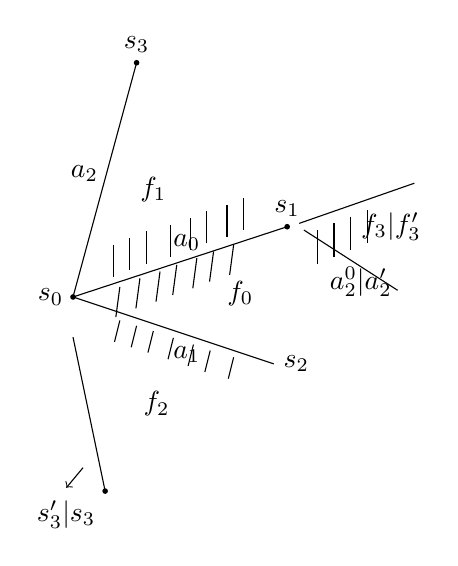
\begin{tikzpicture}[scale=.85]
\coordinate (s0) at (0,0);
\coordinate (s1) at (3.2,1.05);
\coordinate (s2) at (3,-1);
\coordinate (s3) at (.95,3.5);
\coordinate (s3b) at (.48,-2.9);
\draw (s3)--(s0)--(s1);
\draw (3.38,1.1)--(5.1,1.7);
\draw (3.45,1.0)--(4.85,.1);
\draw (s0)--(s2);
\draw (0,-.6)--(s3b);
\foreach \x/\y in {.6/.3,.85/.4,1.1/.5,1.45/.6,1.75/.7,2/.8,2.3/.9,2.55/1.0}
 {\draw[thin] (\x,\y)--+(0,.48);}
\foreach \x/\y in {.7/.15,1/.28,1.3/.38,1.55/.48,1.85/.58,2.1/.68,2.4/.78}
 {\draw[thin] (\x,\y)--+(-.06,-.45);}
\foreach \x/\y in {.7/-.35,.95/-.43,1.2/-.51,1.5/-.61,1.8/-.71,2.05/-.8,2.4/-.9}
 {\draw[thin] (\x,\y)--+(-.08,-.32);}
\foreach \x/\y in {3.65/1.0,3.9/1.1,4.15/1.2,4.4/1.3}
 {\draw[thin] (\x,\y)--+(0,-.5);}
\fill (s0) circle (1.2pt) (s1) circle (1.2pt) (s3) circle (1.2pt) (s3b) circle (1.2pt);
\node[left] at (s0) {$s_0$}; \node[above] at (s1) {$s_1$};
\node[right] at (s2) {$s_2$}; \node[above] at (s3) {$s_3$};
\node[below left] at (s3b) {$\unsure{s'_3|s_3}$};
\draw[->] (.15,-2.55)--(-.1,-2.85);
\node[above] at (1.7,.55) {$a_0$}; \node[below] at (1.7,-.6) {$a_1$};
\node[left] at (.52,1.85) {$a_2$}; \node[below] at (4.3,.6) {$\unsure{a_2^0|a_2'}$};
\node at (2.5,.05) {$f_0$}; \node at (1.2,1.6) {$f_1$};
\node at (1.25,-1.6) {$f_2$}; \node at (4.75,1.05) {$\unsure{f_3|f'_3}$};
\end{tikzpicture}}

% L16-18, right of drawing
et enfin
\[
\begin{aligned}
s_0&=a_0\cap a_1\\
f_0&=\mathrm{pl}(a_0,a_1)
\end{aligned}
\mathrel{\big|\!\!\Longrightarrow}
\begin{gathered}
\varphi_S,\varphi_F\ \text{connus}\\
\text{quand on}\\
\text{\unsure{connaît|connait} }\varphi_A
\end{gathered}
\]

% L19
\uline{Corollaire} $\unsure{S|\mathscr{S}}=\varphi_S(\underline{S})$ engendre aff\textsuperscript{t} $E$.

% L20-21
Réalisation géom \uline{régulière} (si $\underline{X}$ \uline{régulier})
\[
\forall\underline{g}\in\underline{\unsure{G|C}}\overset{\unsure{\mathrm{df}|\mathrm{déf}}}{=}\mathrm{Aut}(X),\quad
\exists g\in\mathrm{Aut}_{\text{aff ou proj}}(E)
\]
% archive sheet number: 52

\scanpage{54}
% L01
tel que \deleted{$g\circ\varphi_S$} l'on ait
% L02-04
\[
\left\{\begin{aligned}
g\circ\varphi_S&=\varphi_S\circ\underline{\unsure{\widetilde{g}|\widehat{g}}}\\
g\circ\varphi_A&=\varphi_A\circ\underline{\widetilde{g}}\\
g\circ\varphi_F&=\varphi_F\circ\underline{\widetilde{g}}
\end{aligned}\right.
\]

% L05-15
\uline{NB} l'une quelc. de ces trois relations implique les deux autres. Dans le cas affine, $\widetilde{g}$ défini de façon unique par $g$, et ainsi $\unsure{G|C}$ opère sur $E$. C'est encore vrai dans le cas projectif, \uline{pourvu que} $\exists\underline{s}\in\underline{S}$ avec $\varphi_S(\underline{s})\deleted{\unsure{\varphi|\ne|s}}=s$ non coplanaire avec trois des quatre pts $s_0\ s_1\ s_2\ s_3$ (unique exception: \deleted{tétraèdre à \unsure{imag.} \unsure{cop}} $S=\{s_0,s_1,s_2,s_3\}$ \ldots)
% slanted
\margin{à vérifier}
Si on veut éliminer ce \unsure{canular|cas-là}, il faut se \uline{donner} $\underline{g}\mapsto g$ faisant opérer $G$ sur $E$ \ldots
% Both ellipses above are visible manuscript continuation dots.

% L16-18
Dorénavant on suppose $\underline{X}$ régulier, on choisit repère $\underline{r}_0=(\underline{s}_0,\underline{a}_0,\underline{f}_0)$, ainsi que $\underline{\sigma}_0,\underline{\sigma}_1,\underline{\sigma}_2$ de $\underline{G}=\mathrm{Aut}(\underline{X})$, définis par
\deleted{$\unsure{\underline{\sigma}_0|\underline{r}_0}$}
% archive sheet number: 53

\scanpage{55}
% L01-03
\[
\left\{\begin{aligned}
\underline{\sigma}_0(\underline{s}_0)&\overset{\unsure{\mathrm{df}|\mathrm{dfn}|\mathrm{déf}}}{=}\underline{s}_1,
&\underline{\sigma}_0(\underline{a}_0)&=\underline{a}_0,
&\underline{\sigma}_0(\underline{f}_0)&=f_0\\
\underline{\sigma}_1(\underline{s}_0)&=\underline{s}_0,
&\underline{\sigma}_1(\underline{a}_0)&\overset{\mathrm{df}}{=}\underline{a}_1,
&\underline{\sigma}_{\unsure{2|1}}(\underline{a}_0)&=\underline{a}_0\\
\underline{\sigma}_2(\underline{s}_0)&=\underline{s}_0,
&\underline{\sigma}_2(\underline{a}_0)&=\underline{a}_0,
&\underline{\sigma}_2(\underline{f}_0)&\overset{\mathrm{df}}{=}\underline{f}_1
\end{aligned}\right.
\]

% L04-08
La donnée de $\varphi$ régulière équivaut à la donnée de $\varphi_G:\underline{\unsure{G|C}}\mathrel{\unsure{-|\longrightarrow}}\mathrm{Aut}(E)$ et $\varphi_{\unsure{\mathscr{R}|\mathcal{R}|R}}(\underline{r}_0)=(s_0,a_0,f_0)\in\mathrm{Drap}_{0,1,2}(E)$, satisfaisant certaines conditions. La donnée de $\varphi_G$ à son tour équivaut à la donnée des
% L09
\[
\sigma_0,\sigma_1,\sigma_2\in\mathrm{Aut}(E)
\]
% L10
satisfaisant certaines conditions, qu'on va expliciter.

% L11-13
Notons qu'indépendamment de la condition de régularité et du \deleted{\unsure{choix}} choix de $\underline{r}_0\in\underline{\mathscr{R}}$, la donnée de $\varphi$ implique
% L14
\[
\varphi_{\mathscr{R}}:\mathscr{R}\mathrel{\unsure{-|\longrightarrow}}\mathrm{Drap}_{012}(E)
\]
% L15-20
qui, dans le cas régulier, doit être une $G$-application, et qui permet de récupérer $\varphi_S,\varphi_A$ et $\varphi_F$ par passage au quotient. Dans le cas \deleted{\unsure{non}} régulier, comme $\mathscr{R}$ est un $G$-torseur, la donnée de $\varphi_{\mathscr{R}}$ équivaut à la donnée de $\varphi_{\mathscr{R}}(\underline{r}_0)\deleted{\unsure{\in|=}}r_0=(s_0,a_0,f_0)$.
% archive sheet number: 54

\scanpage{56}
% L01-02
Pour que la \deleted{\unsure{bonne}} $\unsure{G|C}$-application \unsure{convienne} $\pi_E^{(i)}\circ\varphi_{\unsure{\mathscr{R}|\mathcal{R}|R}}$ passe au quotient \inserted{$\mathrm{Fac}_i(X)\ (=\underline{S},\underline{A},\underline{F})$}, il faut et s. que
% L03-05
\diagram{\begin{tikzcd}[ampersand replacement=\&]
\underline{\mathscr{R}} \arrow[r,"\varphi_{\mathscr{R}}"] \arrow[d,"\pi_{\underline{X}}^{(i)}"']
\& \mathrm{Drap}_{012}(E) \arrow[d,"\pi_E^{(i)}"] \\
\mathrm{Fac}_i(X) \arrow[r] \& \mathrm{Fac}_i(E)
\end{tikzcd}}
\[i=0,1,2\]

% L06-07
\deleted{$\unsure{(s_0,f_0)}$ \unsure{l'image}} le stabilisateur dans $G$ de $\unsure{f_0^{(i)}|\underline{f}_0^{(i)}}$ contienne celui de $f_0^{(i)}$, ce qui s'écrit
% L08-10
\[
\begin{aligned}
\deleted{\unsure{\sigma_0(s_0|\sigma_0(r_0}}\qquad
&\sigma_0(a_0)=a_0 &&\sigma_0(f_0)=f_0\\
\sigma_1(s_0)=s_0
&&&\sigma_1(f_0)=f_0\\
\sigma_2(s_0)=s_0\qquad
&\sigma_2(a_0)=a_0
\end{aligned}
\]
% archive sheet number: 55

\scanpage{57}
% Top right heading
\uline{À vérifier}:

% L01
Cartes \inserted{\unsure{connexes}} homogènes de type $(p,q)$

% L02-04
 a) est \inserted{\unsure{resp.}} géom. d'incidence sauf si
\[
\begin{aligned}
(p\unsure{,|\ne}q)&=(1,2)\\
&\text{\unsure{ou|\textquotedblright} }(2,1)
\end{aligned}
\]
(\unsure{seuls cas où} \unsure{on n'a pas|p ou q} $(p,q)\ge(2,2)$)

% Two small drawings between a) and b)
\figure{\begin{tikzpicture}
\draw (0,1.1) .. controls (-.1,.65) and (-.1,.35) .. (0,0);
\fill (0,1.1) circle (1.8pt) (0,0) circle (1.8pt);
\draw (3.7,.55) .. controls (3.65,1.35) and (2.25,1.05) .. (2.25,.45)
 .. controls (2.3,-.15) and (3.55,-.05) .. (3.7,.55);
\fill (3.7,.55) circle (2pt);
\end{tikzpicture}}

% L05-06
b) est polyèdre combinatoire sauf si
\[p=\unsure{2|3}\ \text{ou}\ q=2\]

% L07
\deleted{c) \unsure{est}}

% L08-09
\[
\left[\begin{aligned}
&\text{C'est une géom d'incidence ssi }(p,q)\ge(2,2)\\
&\text{i.e.}\quad p\ne1,q\ne1\quad\text{i.e.}\quad(p,q)\ne(1,2),(2,1)
\end{aligned}\right.
\]
% L10-12
\[
\left[\begin{aligned}
&\text{C'est un polyèdre combinatoire ssi}\\
&(p,q)\ge(3,3)\quad\text{i.e. ssi}\quad p\ne2,q\ne2,\quad\text{i.e. ssi}\\
&(p,q)\ne(2,q)\ (q\ge1)\quad\text{et}\quad(p,q)\ne(p,2)\ (p\ge1).
\end{aligned}\right.
\]
% archive sheet number: 56

\scanpage{58}
% Entire letter written sideways; crossed out with several long diagonal strokes.
% L01, salutation
\deleted{Cher Wilbert,}\\
% L02-10, body
\deleted{Merci pour votre lettre et les documents joints. Sauf cas de force majeure --- auquel cas il faudrait que vous en reparliez --- je \unsure{préfèrerais|préférerais} ne pas m'engager à assurer la direction d'une thèse de doctorat d'\unsure{État|état} --- chose qui me paraît prématurée, alors que pour le moment il n'y a pas encore de sujet de thèse à l'horizon. Comme je le dis dans l'attestation ci-jointe}
% archive sheet number: 57

\scanpage{59}
% L01-03, upper groupoid notes
$\unsure{C|\mathcal{C}|\mathscr{C}}$ groupoïde.
$G\inserted{\subset\mathrm{Aut}(C)}$ transitif sur $C_0=\mathrm{Ob}\,C$\quad $e\in C_0$\quad $H=G_e$

$\Gamma$ normalisateur de $G$.
$\Gamma^{\unsure{0|\circ}}$ centralisateur de $\unsure{G|C}$.
\[C_0\simeq G/H\]
% L04
\diagram{\begin{tikzcd}[ampersand replacement=\&]
1\arrow[r]\&\Gamma^0\arrow[r]\&\Gamma\arrow[r]\&\mathrm{Aut}(G)
\end{tikzcd}}
% L05-06
$e\in\mathrm{Ob}\,C=C_0$

$\gamma_{C_0}$ connu quand on \unsure{connaît|connait} $\gamma.e$
% L07-08
\diagram{\begin{tikzcd}[ampersand replacement=\&]
1\arrow[r,no head]\&\Gamma^{\deleted{\unsure{2|1}}\unsure{1|2}}\arrow[r,no head]\arrow[d,no head,"\unsure{f}"']\arrow[dr]\&\Gamma^0\arrow[r]\&N(H)/H\\
\&\unsure{H}\&\mathrm{Aut}_H(\pi_e)
\end{tikzcd}}
\figure{\begin{tikzpicture}
\draw (0,0) .. controls (.12,1) and (.35,1.7) .. (.6,2.2);
\draw[->,very thick] (0,0)--(2,1.25) node[midway,above] {$f$};
\fill (0,0) circle (2pt) (.6,2.2) circle (2pt) (2,1.25) circle (2pt);
\node[below] at (0,0) {$e$};
\draw (3.6,.1) .. controls (4.4,1) and (5.3,1.3) .. (6.1,1.6);
\fill (3.6,.1) circle (1.8pt); \node[below] at (3.6,.1) {$\gamma e$};
\end{tikzpicture}}
\par\noindent\rule{\linewidth}{.4pt}

% L09-11, graph notes
$K=K_0,K_1,\ K_1\longrightarrow K_0\ \unsure{\mathrm{inv}}$ (graphe \inserted{connexe}), $G$ grp, \deleted{d'automorphismes de} \inserted{opérant sur} $K$ on suppose que $G$ est transitif sur l'ens $K_1$ des arcs de $K$
% L12-13
\diagram{\begin{tikzcd}[ampersand replacement=\&]
K_1\simeq G/\unsure{H|\mathbb{H}}_1\arrow[d]\\
K_0=G/H_0
\end{tikzcd}}
\[\sigma\in N(H)/H\qquad\sigma^2=1\]

% L14
$C\inserted{=(C_0,C_1)}$ groupoïde, $\deleted{\unsure{C}}$ $G$ opère sur $C_0$
% L15
\diagram{\begin{tikzcd}[ampersand replacement=\&]
\unsure{K_\alpha|K}\arrow[r,hook]\&C
\end{tikzcd}}
$G$-morphisme on suppose
\diagram{\begin{tikzcd}[ampersand replacement=\&]
K_0\arrow[r,"{\deleted{\unsure{\mathrm{équi}}}\ \sim}"]\&C_0
\end{tikzcd}}

% L16, small arrows at left
\figure{\begin{tikzpicture}
\fill (0,0) circle (2pt); \node[below left] at (0,0) {$e$};
\draw[->,very thick] (0,0)--(1.8,.8) node[right] {$e'$};
\node[below left] at (3,-.2) {$\gamma e$};
\draw[->,thick] (3,-.2)--(4.8,.6) node[right] {$\gamma e'$};
\end{tikzpicture}}
% L16-18, lower chains
\diagram{\begin{tikzcd}[ampersand replacement=\&]
1\arrow[r]\&\Gamma^0\arrow[r]\&\Gamma\arrow[r]\&\mathrm{Aut}_*(G)
\end{tikzcd}}
\diagram{\begin{tikzcd}[ampersand replacement=\&]
\Gamma\arrow[r,"\unsure{/}" description]\&G
\end{tikzcd}}
\diagram{\begin{tikzcd}[ampersand replacement=\&]
1\arrow[r]\&\Gamma^1\arrow[r]\&\Gamma^0\arrow[r]\&\deleted{G_*}\arrow[r]\&N(H_0)/H_0
\end{tikzcd}}
\diagram{\begin{tikzcd}[ampersand replacement=\&]
\deleted{1}\arrow[r,no head,"\deleted{\longrightarrow}" description]\&
\deleted{\Gamma^2}\arrow[r,no head,"\deleted{\longrightarrow}" description]\&
\Gamma''\arrow[r,hook]\&\mathrm{Aut}_G\pi_e
\end{tikzcd}}
% L19-20, bottom drawing and notations
\figure{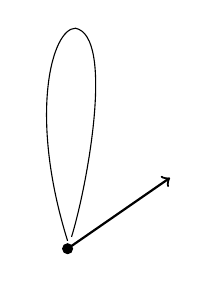
\begin{tikzpicture}
\fill (0,0) circle (2pt);
\draw (0,.1) .. controls (-.5,1.7) and (-.2,2.8) .. (.1,2.8)
 .. controls (.6,2.7) and (.25,.8) .. (.05,.15);
\draw[->,thick] (0,0)--(1.3,.9);
\end{tikzpicture}}
\[
\pi_e,\ \deleted{\unsure{K_e|\Pi_e}}\qquad
\begin{gathered}\mathrm{Hom}(e,e')\\\Vert\\\Pi_{e,e'}\end{gathered}
\qquad\Pi_e\qquad *
\]
\[\unsure{\mathrm{Aff}_{H_0}(\pi_e)|N_{H_0}(\pi_e)}\]
% archive sheet number: 58

\scanpage{60}
% Upper-left lens and adjacent triangular sketch
\figure{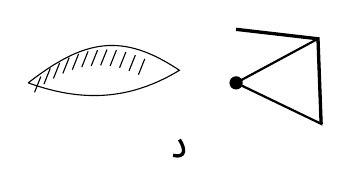
\begin{tikzpicture}[scale=.8]
\draw (0,0) .. controls (.9,.7) and (1.5,.8) .. (2.4,.2)
 .. controls (1.5,-.35) and (.7,-.25) .. (0,0);
\foreach \x/\y in {.2/.1,.35/.23,.5/.32,.65/.4,.8/.46,.95/.5,1.1/.52,1.25/.53,1.4/.52,1.55/.49,1.7/.44,1.85/.38}
 {\draw (\x,\y)--+(-.1,-.25);}
\draw[thick] (3.3,0)--(4.6,.7)--(4.65,-.65)--cycle;
\draw[very thick] (3.3,.85)--(4.6,.7)--(4.65,-.65);
\fill (3.3,0) circle (3pt);
\draw[very thick] (2.3,-1.15).. controls (2.5,-1.2) and (2.5,-1.05)..(2.4,-.9);
\end{tikzpicture}}

% Upper-right labelled fan
\figure{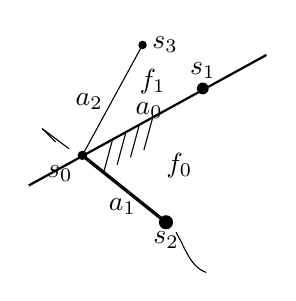
\begin{tikzpicture}[scale=.85]
\coordinate (s0) at (0,0); \coordinate (s1) at (1.8,1);
\coordinate (s2) at (1.25,-1); \coordinate (s3) at (.9,1.65);
\draw[thick] (-.8,-.45)--(2.75,1.5);
\draw (s0)--(s3); \draw[very thick] (s0)--(s2);
\draw (1.4,-1.15)..controls (1.55,-1.4) and (1.6,-1.65)..(1.85,-1.75);
\foreach \x/\y in {.45/.23,.65/.34,.85/.45,1.05/.56}
 {\draw (\x,\y)--+(-.13,-.48);}
\fill (s0) circle (2pt) (s1) circle (2.5pt) (s2) circle (3pt) (s3) circle (1.8pt);
\node[below left] at (s0) {$s_0$}; \node[above] at (s1) {$s_1$};
\node[below] at (s2) {$s_2$}; \node[right] at (s3) {$\unsure{s_3}$};
\node[above] at (1,.4) {$a_0$}; \node[below] at (.6,-.5) {$a_1$};
\node[left] at (.45,.8) {$a_2$};
\node at (1.45,-.15) {$f_0$}; \node at (1.05,1.1) {$f_1$};
\draw (-.6,.4)--(-.2,.1); \draw (-.6,.4)--(-.4,.2);
\end{tikzpicture}}

% Main fan below the top sketches
\figure{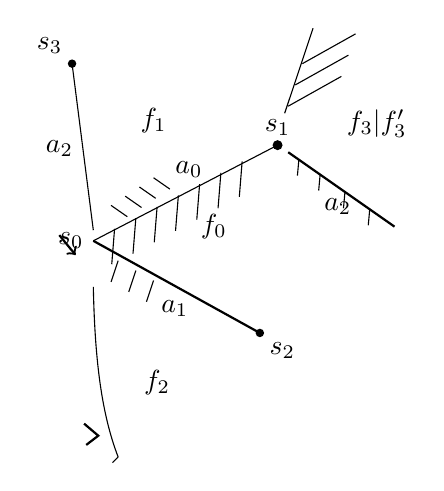
\begin{tikzpicture}[scale=.9]
\coordinate (s0) at (0,0); \coordinate (s1) at (2.6,1.35);
\coordinate (s2) at (2.35,-1.3); \coordinate (s3) at (-.3,2.5);
\draw (s3)--(0,.15); \draw (s0)--(s1);
\draw[thick] (s0)--(s2); \draw[thick] (2.75,1.25)--(4.25,.2);
\draw (2.7,1.8)--(3.1,3.0);
\draw (0,-.65)..controls (.02,-1.6) and (.1,-2.4)..(.35,-3.05);
\foreach \x/\y in {.3/.17,.6/.32,.9/.48,1.2/.64,1.5/.8,1.8/.96,2.1/1.12}
 {\draw[thin] (\x,\y)--+(-.04,-.5);}
\foreach \x/\y in {.25/.5,.45/.63,.65/.76,.85/.89}
 {\draw[thin] (\x,\y)--+(.23,-.16);}
\foreach \x/\y in {.35/-.28,.6/-.42,.85/-.56}
 {\draw (\x,\y)--+(-.1,-.3);}
\foreach \x/\y in {2.9/1.14,3.2/.93,3.55/.68,3.9/.44}
 {\draw (\x,\y)--+(-.02,-.22);}
\foreach \x/\y in {2.75/1.9,2.85/2.2,2.95/2.5}
 {\draw[thin] (\x,\y)--+(.75,.42);}
\fill (s1) circle (2pt) (s2) circle (1.7pt) (s3) circle (1.7pt);
\node[left] at (s0) {$s_0$}; \node[above] at (s1) {$s_1$};
\node[below right] at (s2) {$s_2$}; \node[above left] at (s3) {$s_3$};
\node[above] at (1.35,.75) {$a_0$}; \node[below] at (1.15,-.7) {$a_1$};
\node[left] at (-.15,1.3) {$a_2$}; \node[below] at (3.45,.73) {$a_2$};
\node at (1.7,.2) {$f_0$}; \node at (.85,1.7) {$f_1$};
\node at (.9,-2) {$f_2$}; \node at (4,1.65) {$\unsure{f_3|f'_3}$};
\draw[->,thick] (-.48,.08)--(-.25,-.2);
\draw[thick] (-.13,-2.58)--(.07,-2.75)--(-.1,-2.88);
\draw (.35,-3.05)--(.27,-3.13);
\end{tikzpicture}}
% archive sheet number: 59

\scanpage{62}
% Upper-left sequence, with identifications written beneath it
\diagram{\begin{tikzcd}[ampersand replacement=\&,column sep=small]
1\arrow[r]\&\unsure{\widetilde{R}_\infty|\mathscr{R}_\infty}\arrow[r]\arrow[d,equal]\&
\mathrm{SL}(2,\mathbb{Z})/\unsure{\{\pm1\}|\{1\}}\arrow[r]\arrow[d,equal]\&
\mathrm{SL}(2,\mathbb{Z}_2)\arrow[r]\arrow[d,equal]\&0\\
\&\widetilde{R}(\infty,2,2,3)\&\Gamma^{\unsure{0|\circ}}_{\infty,3}\&\unsure{\mathfrak{S}_3|G_3}\arrow[d,equal]\\
\&\&\&\Gamma_{2,3}
\end{tikzcd}}
% Upper-left text and formula
engendré par
\[\rho_s^2=(\sigma\rho_f^{-1})^2\]
% Upper-right identities
\[
\left\{\begin{aligned}
\rho_s&=\sigma_0\sigma_1\\
\rho_f&=\sigma_1\sigma_2\\
\rho_s\rho_f&=\sigma_0\sigma_2=\sigma
\end{aligned}\right.
\qquad\rho_s=\sigma\rho_f^{-1}
\]
\[\boxed{\begin{aligned}\rho_f^3&=1\\\sigma^2&=1\end{aligned}}\]

% L05-08
\[
\frac{az+b}{cz+d}=z\qquad cz^2+(d-a)z-b=0\qquad z=x+iy\quad(y\ne0)
\]
\[
\left\{\begin{aligned}
c(x^2\unsure{-|+}y^2)+(d-a)x-b&=0\\
[2cx+(d-a)]y&=0\quad\Longleftrightarrow\quad2cx+(d-a)=0
\end{aligned}\right.
\]
\[
\Updownarrow\quad
\left\{\begin{aligned}d-a&=-2cx\\-c(x^2+y^2)\unsure{+|-}b&=0\end{aligned}\right.
\qquad
\left|\begin{aligned}d&=a-c\mathrm{Tr}(z)\\b&=-cN(z)\end{aligned}\right.
\]
% L09-10
\[
\begin{pmatrix}a&b\\c&d\end{pmatrix}
=\begin{pmatrix}a&-cN(z)\\c&a-c\mathrm{Tr}z\end{pmatrix}
\]
\[
\det=a^2-ac\mathrm{Tr}z+c^2N(z)=(a-cz)(a-c\bar{z})=N(a-cz)=1
\]

% L11-14
1°) $z=i$\quad $\mathrm{Tr}z=0,\ N(z)=1$\quad ($z$ racine primitive 4\textsuperscript{ième} de 1)
\[
G_z=G_i=\left\{\begin{pmatrix}a&-c\\c&a\end{pmatrix}\,\middle|\,a^2+c^2=1\right\}
\]
élément d'ordre 4
\[
\boxed{\sigma=\begin{pmatrix}0&-1\\1&0\end{pmatrix}}
\qquad\sigma^4=\mathrm{id}\qquad\boxed{\sigma^2=-\unsure{1_E|\mathrm{id}|\mathrm{Id}}}
\]

% L15-17
2°) $z=\dfrac12+i\dfrac{\sqrt3}{2}=\zeta$\quad ($z$ racine primitive 6\textsuperscript{ème} de 1)
\[\mathrm{Tr}z=1,\quad Nz=1\]
\[
G_z=G_\zeta=\left\{\begin{pmatrix}a&-c\\c&a-c\end{pmatrix}\,\middle|\,a^2-ac+c^2=1\right\}
\]
\[N(a-c\unsure{\zeta|z})=1\]
% L18-19, overwritten signs before the matrix entries
\[
\deleted{\unsure{\rho_s|\rho}}\mathrel{\unsure{=}}
\boxed{\rho_f=\begin{pmatrix}0&\deleted{\unsure{-}}1\\-1&\deleted{\unsure{-}}1\end{pmatrix}}
\quad\deleted{\unsure{\rho}}\quad\rho^6=\mathrm{id}\qquad\boxed{\rho^3=-1_E}
\]
% L20-21
\[
\boxed{\begin{gathered}
\rho_s'=\sigma\rho_f=\begin{pmatrix}1&-1\\0&1\end{pmatrix}\\
\Vert\\
\sigma_2\rho_f\sigma_2^{-1}
\end{gathered}}
\qquad
\rho_s'{}^n=\begin{pmatrix}1&-n\\0&1\end{pmatrix}
\]
% archive sheet number: 61

\scanpage{63}
% L01
\[\Gamma^{\unsure{0|\circ}}_{\infty,3}\simeq\mathrm{SL}(2,\mathbb{Z})/\pm1\]
% L02-03
\diagram{\begin{tikzcd}[ampersand replacement=\&]
\Gamma^0_{n,3}\arrow[r,"\text{épi}"]\&\mathrm{SL}(2,\mathbb{Z}_n)/\pm1\arrow[d,equal]\\
\&\deleted{\unsure{\mathrm{GL}(2,\mathbb{Z}_n)|\mathrm{PSL}(2,\mathbb{Z}_n)}}
\end{tikzcd}}
$(n\ge\unsure{2|3})$ (iso \uline{ssi $n\le5$})
% Rounded marginal callout, with its tail towards the condition n<=5.
\margin{\figure{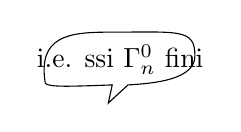
\begin{tikzpicture}[x=1cm,y=1cm]
\draw (0,.2)..controls (-.1,.8) and (.3,.85)..(.8,.85)
 ..controls (1.7,.85) and (1.9,.9)..(1.9,.55)
 ..controls (1.9,.25) and (1.4,.2)..(1.05,.18)
 --(.8,-.05)--(.85,.18)
 ..controls (.3,.16) and (.05,.15)..(0,.2);
\node[align=center] at (.95,.5) {i.e. ssi $\Gamma_n^0$ fini};
\end{tikzpicture}}}
% L04-05
l'étudier pour $n=$\uline{$2,3,4,5,6$}

% Above table, cancelled heading
\deleted{ordre $\Gamma_{n,3}$}
% L06-11, table
\diagram{$\begin{array}{c|l|c|l}
n&\text{ordre }\Gamma^0_{n,3}&\text{ordre }\mathrm{SL}(2,\unsure{\mathbb{Z}/n|\mathbb{Z}_n|\mathbb{Z}/n\mathbb{Z}})/\pm1&\\\hline
2&(\unsure{\mathfrak{S}_3|G_3})\ 6&6&\text{cas 3-dièdre?}\\\hline
3&(\unsure{\mathfrak{A}_4|\mathcal{A}_4})\ 12&12&\text{tétraèdre }\unsure{\text{or.}|\text{or}}\\\hline
4&(\mathfrak{S}_4)\ 24&24&\text{\uline{cube orienté}}\\\hline
5&(\mathfrak{A}_5)\ 60&60&\text{icos. orienté}\\\hline\hline
6&(\mathbb{Z}_6\cdot\mathbb{Z}^2)\ \infty&72&\begin{gathered}\text{pav. en }\unsure{\text{triangles}}\\\text{\uline{\unsure{équilat.} orienté}}\\\text{\uline{du plan}}\end{gathered}
\end{array}$}

% Right of table, upper formula
\[
\begin{aligned}
\operatorname{Card}\mathrm{SL}(2,\mathbb{F}_q)&=(q+1)q(q-1)\\
&=q(q^2-1)
\end{aligned}
\]
% Right of table, lower formula
\[
\begin{aligned}
\operatorname{Card}\mathrm{SL}(2,\mathbb{Z}/p^{\unsure{n|\nu}}\mathbb{Z})&=\\
(\operatorname{card}\mathrm{SL}(2,\mathbb{F}_p))\,p^{3(n-1)}&
\end{aligned}
\]
% archive sheet number: 62

\scanpage{65}
% L01-04, top relations
\[\sigma_0\quad\sigma_1\quad\sigma_2\]
\[r=(s_0,a_0,f_0)\]
\[
\begin{aligned}
\sigma_0s_0&=s_1&\sigma_0a_0&=a_0&\sigma_0f_0&=f_0\\
\sigma_1s_0&=s_0&\sigma_1a_0&=\{s_0,s_2\}&\sigma_1f_0&=f_0\\
\sigma_2s_0&=s_0&\sigma_2a_0&=a_0&\sigma_2f_0&=\{s_0,s_1,s_3\ldots\}
\end{aligned}
\qquad
\begin{aligned}a_0&=\{s_0,s_1\}\\f_0&=\{s_0,s_1,s_2\ldots\}\end{aligned}
\]
% L05-07, left of main drawing
\[\begin{aligned}\sigma_0s_0&=s_1\\\sigma_1s_1&=s_2\\\sigma_2s_2&=s_3\end{aligned}\]
% Main drawing
% crop-candidate: scan 65
\figure{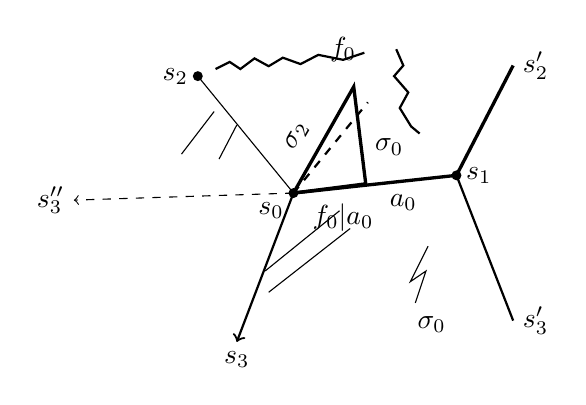
\begin{tikzpicture}[scale=.9]
\coordinate (s0) at (0,0); \coordinate (s1) at (2.3,.25);
\coordinate (s2) at (-1.35,1.65); \coordinate (s3) at (-.8,-2.1);
\coordinate (s2p) at (3.1,1.8); \coordinate (s3p) at (3.1,-1.8);
\draw (s2)--(s0); \draw[thick,->] (s0)--(s3);
\draw[very thick] (s0)--(s1)--(s2p); \draw[thick] (s1)--(s3p);
\draw[->,dashed] (s0)--(-3.1,-.1);
\draw[very thick] (s0)--(.85,1.5)--(1.02,.13)--cycle;
\draw[dashed,thick] (s0)--(1.05,1.28);
\draw[thin] (-1.58,.55)--(-1.12,1.15); \draw[thin] (-1.05,.48)--(-.8,.96);
\draw[thin] (-.4,-1.1)--(.65,-.25); \draw[thin] (-.35,-1.4)--(.8,-.5);
\draw[thick] (-1.1,1.75)--(-.9,1.85)--(-.75,1.75)--(-.55,1.9)--(-.35,1.79)--(-.15,1.91)--(.1,1.82)--(.35,1.95)--(.7,1.88)--(1,1.98);
\draw[thick] (1.45,2.03)--(1.55,1.8)--(1.42,1.65)--(1.62,1.42)--(1.5,1.2)--(1.66,.94)--(1.78,.84);
\draw (1.9,-.75)--(1.65,-1.25)--(1.87,-1.1)--(1.72,-1.55);
\fill (s2) circle (2pt) (s0) circle (2pt) (s1) circle (2pt);
\node[below left] at (s0) {$s_0$}; \node[right] at (s1) {$s_1$};
\node[left] at (s2) {$s_2$}; \node[below] at (s3) {$s_3$};
\node[right] at (s2p) {$s'_2$}; \node[right] at (s3p) {$s'_3$};
\node[left] at (-3.1,-.1) {$s''_3$};
\node[below] at (1.55,.12) {$a_0$};
\node at (.7,2.03) {$\deleted{\unsure{f_0}}$};
\node[rotate=60] at (.05,.8) {$\unsure{\sigma_2}$};
\node at (1.35,.65) {$\sigma_0$};
\node at (.7,-.35) {$\deleted{\unsure{f_0|a_0}}$};
\node at (1.95,-1.85) {$\unsure{\sigma_0}$};
\end{tikzpicture}}
% L05-07, right of main drawing
\[
\left\{\begin{aligned}e_1&=s_1-s_0\\e_2&=s_2-s_0\\e_3&=s_3-s_0\end{aligned}\right.
\]
% L08-11, three action lists
\[
\sigma_0\left\{\begin{aligned}s_0&\longmapsto s_1\\s_1&\longmapsto s_0\\s_2&\longmapsto s'_2\\s_3&\longmapsto s'_3\end{aligned}\right.
\quad
\sigma_1\left\{\begin{aligned}s_0&\longmapsto s_0\\s_1&\longmapsto s_2\\s_2&\longmapsto s_1\\s_3&\longmapsto s''_3\end{aligned}\right.
\quad
\sigma_2\left\{\begin{aligned}s_0&\longmapsto s_0\\s_1&\longmapsto s_1\\s_2&\longmapsto s_3\\s_3&\longmapsto s_2\end{aligned}\right.
\]
% Isolated cancelled symbol between action lists and plane equalities
\[\deleted{\unsure{\sigma_2}}\]
% L08-11, boxed notes at right
\[
\boxed{\begin{gathered}\mathrm{Pl}(s_0,s_1,s_2)\\\deleted{\unsure{(s_0,s_1,s_0)}}\\=\mathrm{Pl}(s_0,s_1,s'_2)\end{gathered}}
\]
\[\boxed{\mathrm{Pl}(s_0,s_1,s_3)=\mathrm{Pl}(s_0,s_1,s'_3)}\]

% L12-16, commuting relation and comparison table
\diagram{\begin{tikzcd}[ampersand replacement=\&]
\begin{gathered}
\boxed{\sigma_0\sigma_2=\sigma_2\sigma_0}\\
\begin{array}{c|cc}
s_0\mapsto&s_1&s_1\\
s_1\mapsto&s_0&s_0\\
s_2\mapsto&s'_3&\sigma_2s'_2\\
s_3\mapsto&s'_2&\sigma_2s'_3
\end{array}
\end{gathered}\arrow[dr,Leftrightarrow]\&\\
\&\begin{gathered}\boxed{\sigma_2s'_2=s'_3}\\\sigma_2s'_3=s'_2\end{gathered}
\end{tikzcd}}
% L12-14, involution conditions to the right
\diagram{\begin{tikzcd}[ampersand replacement=\&]
\boxed{\sigma_0^2=1}\arrow[dr,Leftrightarrow]\&\\
\&\boxed{\begin{aligned}\sigma_0s'_2&=s_2\\\sigma_0s'_3&=s_3\end{aligned}}
\end{tikzcd}}
\diagram{\begin{tikzcd}[ampersand replacement=\&]
\boxed{\sigma_1^2=1}\arrow[dr,Leftrightarrow]\&\\
\&\boxed{\sigma_1s''_3=s_3}
\end{tikzcd}}
\[\sigma_2^2=1\quad\text{automatique}\]

% L17, linked by the curved double arrow to sigma_2 s'_2=s'_3 above
\diagram{\begin{tikzcd}[ampersand replacement=\&,row sep=small]
{}\arrow[d,bend left=35,Leftrightarrow]\\{}
\end{tikzcd}}
% Coordinate tuples are added above the right ends of the two expressions.
\[
s'_2=s_0+\lambda e_1+\mu e_2\inserted{=(\lambda,\mu,0)}
\qquad s'_3=s_0+\lambda e_1+\mu e_3\inserted{=(\lambda,0,\mu)}
\]
\[
\left[\underbrace{\mu=1}_{?},\ \lambda=1+\beta\ldots\right.
\]
% L18-19
\[
\begin{aligned}
s''_3&=s_3+\xi e_1+\eta e_2+\zeta e_3\\
&=s_0+\xi e_1+\eta e_2+(1+\zeta)e_3=(\xi,\eta,1-\zeta)
\end{aligned}
\]
\[
\left[\underbrace{\unsure{\xi|\zeta}=-\eta}_{?},\ \eta=1+\alpha,\ \underbrace{\zeta=0}_{?}\right.
\]
% Lower-left drawing
\figure{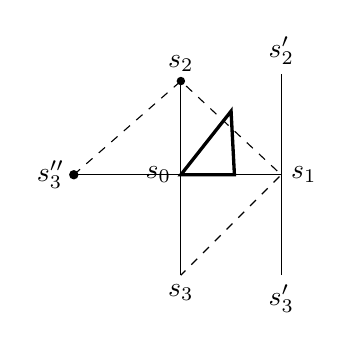
\begin{tikzpicture}[scale=.85]
\draw (0,-1.5)--(0,1.4); \draw (1.5,-1.5)--(1.5,1.5);
\draw (-1.6,0)--(1.5,0);
\draw[dashed] (-1.6,0)--(0,1.4)--(1.5,0)--(0,-1.5);
\draw[very thick] (0,0)--(.75,.95)--(.8,0)--cycle;
\fill (-1.6,0) circle (2pt) (0,1.4) circle (1.8pt);
\node[left] at (-1.6,0) {$s''_3$}; \node[left] at (0,0) {$s_0$};
\node[above] at (0,1.4) {$s_2$}; \node[below] at (0,-1.5) {$s_3$};
\node[right] at (1.5,0) {$s_1$}; \node[above] at (1.5,1.5) {$s'_2$};
\node[below] at (1.5,-1.5) {$s'_3$};
\end{tikzpicture}}
% L20-23
\[
\left\{\begin{aligned}
\sigma_0s_0&=s_1=(1,0,0)\\
\sigma_0e_{\unsure{0|1}}&=-e_1\\
\sigma_0e_2&=(\lambda-1)e_1+\mu e_2\\
\sigma_0e_3&=(\lambda-1)e_1+\mu e_3
\end{aligned}\right.
\]
% L24
\[
\sigma_0=\begin{pmatrix}
-1&\lambda-1&\lambda-1&1\\
0&\mu&0&0\\
0&0&\mu&0\\
0&0&0&1
\end{pmatrix}
\]
% archive sheet number: 64

\scanpage{66}
% L01
\[\boxed{\sigma_0(x,y,z)=(1-x+(\lambda-1)y+(\lambda-1)z,\ \mu y,\ \mu z)}\]
% L02-03, the question mark stands beside a vertical equality
\[
\begin{gathered}
\sigma_0(s'_2)=\sigma_0(\lambda,\mu,0)=(1-\lambda+(\lambda-1)\mu,\mu^2,0)\ \deleted{\unsure{=|?}}\\
?\;\Vert\\s_2=(0,1,0)
\end{gathered}
\]
% L04-06, equivalences drawn diagonally between the blocks
i.e.
\diagram{\begin{tikzcd}[ampersand replacement=\&]
\&{}\arrow[dl,Leftrightarrow,end anchor=north east]\\
\boxed{\mu^2=1\quad(\lambda-1)(\mu-1)=0}\arrow[d,Leftrightarrow,start anchor=south west,end anchor=north west]\&\\
\begin{gathered}
\sigma_0(s'_3)=s_3\ \deleted{\unsure{\sigma_2|?}}\quad\text{i.e.}\quad
\begin{array}{ccc}
\sigma_2\sigma_0(s'_3)&=&\sigma_2s_3\\
\Vert&&\Vert\\
\sigma_0\sigma_2s'_3=\sigma_0s'_2&&s_2
\end{array}
\end{gathered}\&
\end{tikzcd}}
% L07-10, cancelled beginning to the left of the brace
\[
\deleted{\unsure{\sigma_1s''_3|\sigma_1s_3}}
\left\{\begin{aligned}
\sigma_1s_0&=s_0=(0,0,0)\\
\sigma_1e_1&=e_2\\
\sigma_1e_2&=e_1\\
\sigma_1e_3&=\deleted{\unsure{\xi|\zeta}}\xi e_1+\eta e_2+(1+\zeta)e_3
\end{aligned}\right.
\qquad
\sigma_1=\begin{pmatrix}
0&1&\xi&0\\1&0&\eta&0\\0&0&1+\zeta&0\\0&0&0&1
\end{pmatrix}
\]
% L11
\[\boxed{\sigma_1(x,y,z)=(y+\xi z,x+\eta z,(1+\zeta)z)}\]
% L12-13
\[
\begin{gathered}
\sigma_1(s''_3)=\sigma_1(\xi,\eta,1-\zeta)
=(\eta+\xi(1-\zeta),\xi+\eta(1-\zeta),\underbrace{(1+\zeta)(1-\zeta)}_{1-\zeta^2})\\
?\;\Vert\\s_3=(0,0,1)
\end{gathered}
\]
% L14-15
\[\therefore\quad\zeta^2=0,\quad\eta+\xi-\xi\zeta=\eta+\xi-\eta\zeta=0\]
\[\boxed{\zeta^2=0\quad\eta+\xi=\xi\zeta=\eta\zeta}\]
% L16-18
\uline{NB}
\[
\begin{aligned}
\det\sigma_{0V}&=-\mu^2=-1\\
\det\sigma_{1V}&=-(1+\zeta)\\
\det\sigma_{2V}&=-1
\end{aligned}
\qquad\text{donc}\quad
\begin{gathered}
\boxed{(\det\sigma_{1V}=1)\Longleftrightarrow\zeta=0}\\
\Downarrow\\\xi=-\eta
\end{gathered}
\]
% archive sheet number: 65
